% RESULTADOS-------------------------------------------------------------------

\chapter{ANÁLISE E DISCUSSÃO DOS RESULTADOS}

\label{chap:resultados}
% Cada capítulo deve conter uma pequena introdução (tipicamente, um ou dois parágrafos) que deve deixar claro /o objetivo e o que será discutido no ecapítulo, bem como a organização do capítulo.

Nesta seção estão descritos os resultados obtidos a partir dos experimentos realizados na rede neural convolucional proposta, apresentando também os resultados obtidos com as variações das aplicações das técnicas propostas.
 %A métrica utilizada para avaliar os modelos foi a acurácia, que determina a porcentagem de acerto do classificador.%TODO definir melhor a metrica
 Os experimentos foram iniciados a partir da rede neural convolucional sem nenhuma alteração, seguindo para a inclusão das alterações na base e melhorias na rede, com o propósito de avaliar os resultados obtidos e determinar o modelo com a melhor acurácia.

%\par Os experimentos foram executados utilizando máquinas com as seguintes configurações: processado i7  

\par Nos experimentos iniciais realizados foi identificados que a partir de 80 épocas de execução não ocorria nenhuma modificação nas fases de treino e teste, sempre mantendo uma faixa de variação constante. Dessa maneira foi definido como padrão a quantidade de 80 épocas para a execução dos experimentos. A escolha dos parâmetros da rede como a taxa de \textit{dropout}, foram definidos com base na rede descrita por \citeonline{imaginetArticle}. Como abordagem de melhoria a taxa de \textit{dropout} foi otimizada para o modelo proposto com base em testes empíricos.
%\section{Acurácia}


\section{Modelo inicial}
O experimento realizado com o modelo inicial proposto utilizando da base de dados sem modificação obteve um resultado de 94,02\% de acurácia na base de treino e 53,6\% na base de teste, como apresentado na \autoref{tab:resultado1}. Com esses valores é possível dizer que ocorreu um \textit{overfitting} no modelo sobre as amostras da base de treino. Com o gráfico apresentado na \autoref{fig:resultado1} é visto que a acurácia da fase de teste a partir de 42 épocas mantém valores constantes, não apresentando um ganho expressivo, diferente da acurácia obtida na fase de treino que mantém uma curva crescente.

\begin{table}[H]
    \centering
    \caption{Resultado da execução do modelo inicial sem as aplicações das melhorias \textit{data augmentation} e inicialização dos pesos.
    \label{tab:resultado1}}
    \begin{tabular}{ccc}
        \toprule
              & Fase de treino & Fase de Teste \\
        \midrule
            Modelo inicial & 94,02\% & 53,6\%  \\
        \bottomrule
    \end{tabular}
\end{table}


\begin{figure}[H]
  \centering
  \caption{Gráfico contendo a acurácia obtida na fase de treino e teste de cada época do modelo de rede neural inicialmente proposta sem a aplicação de técnicas de melhorias.}
  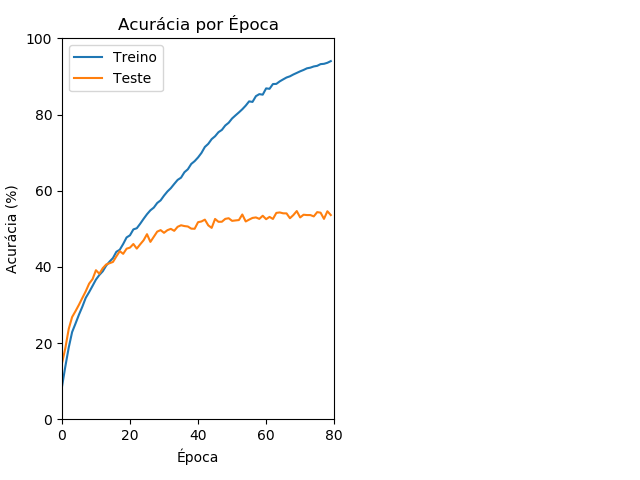
\includegraphics[width=300pt]{dados/figuras/resultado1}
  \label{fig:resultado1}
\end{figure}

\section{Modelos com \textit{data augmentation} e inicialização dos pesos}
Também foram realizados experimentos com as estratégias de melhorias da rede neural, com o objetivo de reduzir o \textit{overfitting} na rede. Foram realizados três experimentos: um aplicando a técnica de \textit{data augmentation}; um a técnica de inicialização dos pesos a partir dos valores treinados na rede \textit{AlexNet} desenvolvida por \citeonline{imaginetArticle}; e um com ambas as técnicas. 

\par Como informado na \autoref{tab:resultado2} as acurácias obtidas na fase de teste e treino, respectivamente, apenas com \textit{data augmentation} foram de 58,23\% e 71,66\%, vendo com essa mudança causou uma redução significativa do \textit{overfitting} na rede, além de uma melhora da acurácia na fase de teste.

\begin{table}[H]
    \centering
    \caption{Resultados da execução do modelo inicialmente proposto sem a aplicação de tecnicas de melhorias.
    \label{tab:resultado2}}
    \begin{tabular}{ccc}
        \toprule
              & Fase de treino & Fase de Teste \\
        \midrule
            Modelo com \textit{data augmentation} & 71,66\% & 58,23\%  \\
            Modelo com inicialização dos pesos & 99,63\% & 68,08\%  \\
            Modelo com \textit{data augmentation} e inicialização dos pesos & 98,18\% & 71,77\%  \\
        \bottomrule
    \end{tabular}
\end{table}


\begin{figure}[H]
  \centering
  \caption{Gráficos contendo as acurácias obtidas nas fases de treino e teste dos modelos com as melhorias aplicadas. No gráfico (1) apresenta os resultados do experimento com a utilização de \textit{data augmentation}. No gráfico (2) apresentado os resultados do experimento com a inicialização dos pesos a partir de uma rede treinada. O gráfico (3) apresenta os resultados obtidos com o modelo com a técnica de \textit{data augmentation} e inicialização dos pesos.}
  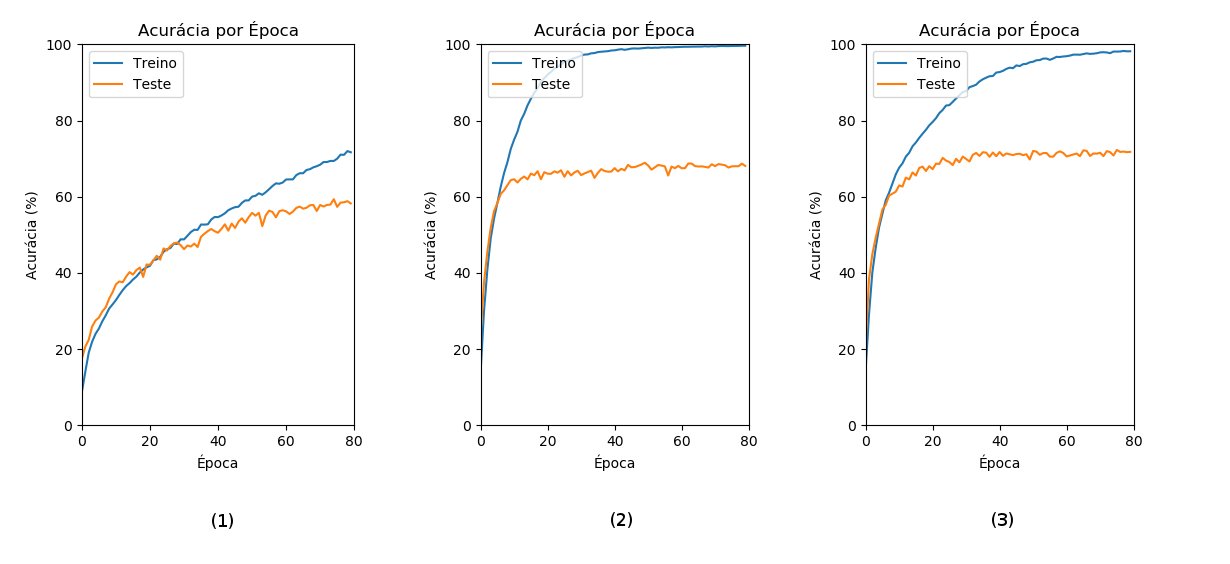
\includegraphics[width=500pt]{dados/figuras/resultado2}
  \label{fig:resultado2}
\end{figure}

\par O experimento realizado com a inicialização dos pesos obteve o resultado mais expressivo se comparado com o teste apenas com \textit{data augmentation} obtendo as acurácias na fase de teste e treino, respectivamente, de 68,08\% e 99,63\%. Com a aplicação dessa técnica foi obtida uma melhora significativa na acurácia se comparado com o modelo inicial e com o de \textit{data augmentation}, mas assim como no modelo inicial esse apresenta \textit{overfitting} na fase de treino, como é possível observar nos gráficos (2) da \autoref{fig:resultado2}, a partir da época 20 a acurácia da fase de teste permanece estável e a fase de treino continua crescendo até atingir valores próximos a 100\%.

\par Com o intuito de solucionar o problema de \textit{overfitting} e obter melhoria na classificação, foi realizado o teste utilizando as duas técnicas. A acurácia obtida na fase de treino foi de 98,18\% e na fase de teste obteve um valor de 71,77\%, apresentando o melhor resultado entre os três testes realizados como pode ser observado no gráfico comparativo na \autoref{fig:resultado2all}.% TODO colocar referencias que apresentam melhoria em modelos aplicados  data augmentantion e inicialização de pesos
\begin{figure}[H]
  \centering
  \caption{Gráficos contendo as acurácias obtidas nas fases de teste dos modelos com as melhorias aplicadas.}
  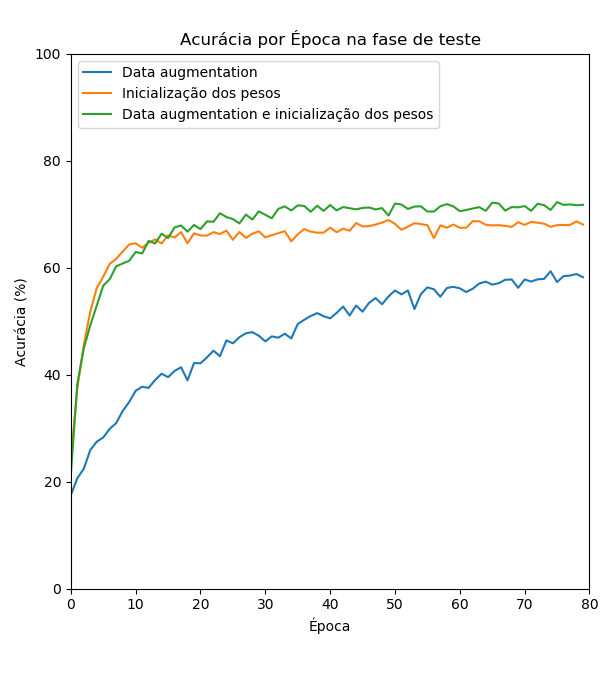
\includegraphics[width=500pt]{dados/figuras/resultado2_all}
  \label{fig:resultado2all}
\end{figure}
 
\section{Aprimoramento da taxa de \textit{dropout}}
Foram realizados experimentos com a taxa de \textit{dropout} buscando diminuir o \textit{overfitting} na rede. A taxa de \textit{dropout} foi variada de 50\% a 90\%, com intervalos de 10\% entre cada experimento. O modelo utilizado para a execução dos foi o com a aplicação de \textit{data augmentation} e inicialização dos pesos. Como pode ser verificado na \autoref{tab:resultado3} que a taxa de 80\% foi a que apresentou melhor resultado, com uma acurácia de 74,56\% na fase de teste e 93,96\% de acurácia na fase de treino.

\begin{table}[H]
    \centering
    \caption{Resultados da execução com a variação na taxa de \textit{dropout}.
    \label{tab:resultado3}}
    \begin{tabular}{ccc}
        \toprule
             Taxa de \textit{dropout} (\%) & Fase de treino & Fase de Teste \\
        \midrule
            Modelo com taxa de 60\% & 97,78\% & 72\%  \\
            Modelo com taxa de 70\% & 96,61\% & 72,77\%  \\
            Modelo com taxa de 80\% & 93,96\% & 74,56\%  \\
            Modelo com taxa de 90\% & 95,37\% & 72,24\%  \\
        \bottomrule
    \end{tabular}
\end{table}


\par A partir da \autoref{tab:resultado3} é possível concluir que o experimento realizado com a taxa de \textit{dropout} 80\% apresentou a maior acurácia na fase de teste e apresentou a menor diferença entre os resultados da fase de treino e teste, conseguindo reduzir o \textit{overfitting} que ocorre na rede. 

